\section{Flyweight}

O padrão Flyweight permite economizar o espaço em memória 
da aplicação ao fornecer uma instância compartilhada de 
uma classe, para que ela não precise ser instanciada 
diversas vezes.

\begin{figure}[htb]
	\caption{\label{flyweight_struct}Estrutura do Flyweight}
	\begin{center}
	    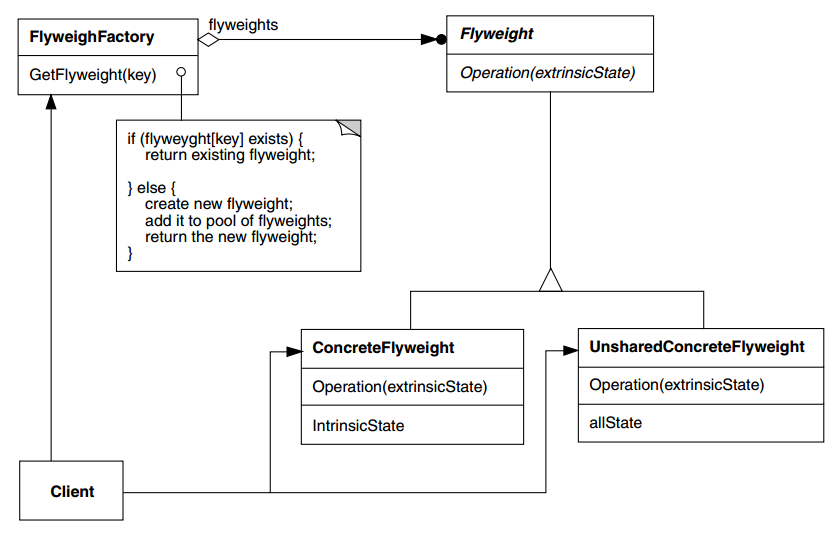
\includegraphics[scale=0.5]{5_padroes-contexto-funcional/5.2_estruturais/5.2.6_flyweight/diagram.png}
	\end{center}
\end{figure}

Exemplo Orientado a Objetos:

\begin{lstlisting}[caption={Flyweight Orientado a Objetos},label=ooflyweight]



\end{lstlisting}

Contexto Funcional:

A ideia do Flyweight assemelha-se à de memoização, onde o 
retorno de uma função pura é armazenado para que seu valor 
não precise ser recalculado quando os mesmos parâmetros 
são passados. Essa abordagem só é possível para funções 
puras pois, caso ocorram efeitos colaterais ou a função 
dependa de dados externos, o resultado pode ser diferente 
para os mesmos parâmetros, gerando um resultado não 
confiável.

Apesar da ideia de memoização parecer mais focada no tempo 
de execução no que no espaço em memória, dependendo da 
implementação é possível economizar ambos.

\begin{lstlisting}[caption={Flyweight Funcional},label=fpflyweight]
    

    
\end{lstlisting}